% Geometry setup
\documentclass[14pt,a4paper]{article}
\usepackage[margin=3cm]{geometry}

% Language setup
\usepackage[magyar]{babel} % Babel for Hungarian
\usepackage[T1]{fontenc} % Output character encoding
\usepackage[utf8]{inputenc} % Input character encoding

% Spacing setup
\setlength{\parindent}{0pt} % No paragraph indenting
\setlength{\parskip}{5pt} % Set spacing between paragraphs
\frenchspacing
\newcommand{\rmspace}{\vspace{-19pt}}

% Dependency setup
\usepackage{amsmath}
\usepackage{amssymb}
\usepackage{listings}
\usepackage{float}
\usepackage{graphicx}
\usepackage{url}

% Python pretty print
\usepackage{minted}
% End Python setup

% Title setup
\title{Nagyadat Coolmini}
\author{Gesztesy Tamás, Nemkin Viktória}
\date{}

% Document
\begin{document}
\maketitle

\section{Bevezetés, feladat}

A félév során a Cool Mini Or Not weboldal (\url{http://www.coolminiornot.com}) adatelemzésével foglalkoztunk.

Az Cool Mini Or Not weboldal egy figurafestésekre specializálódott közösségi oldal, ahova a kifestett miniket
lehet feltölteni, a többi felhasználó pedig szavazhat és kommentelhet a fotóinkra.

\begin{figure}[H]
\centering
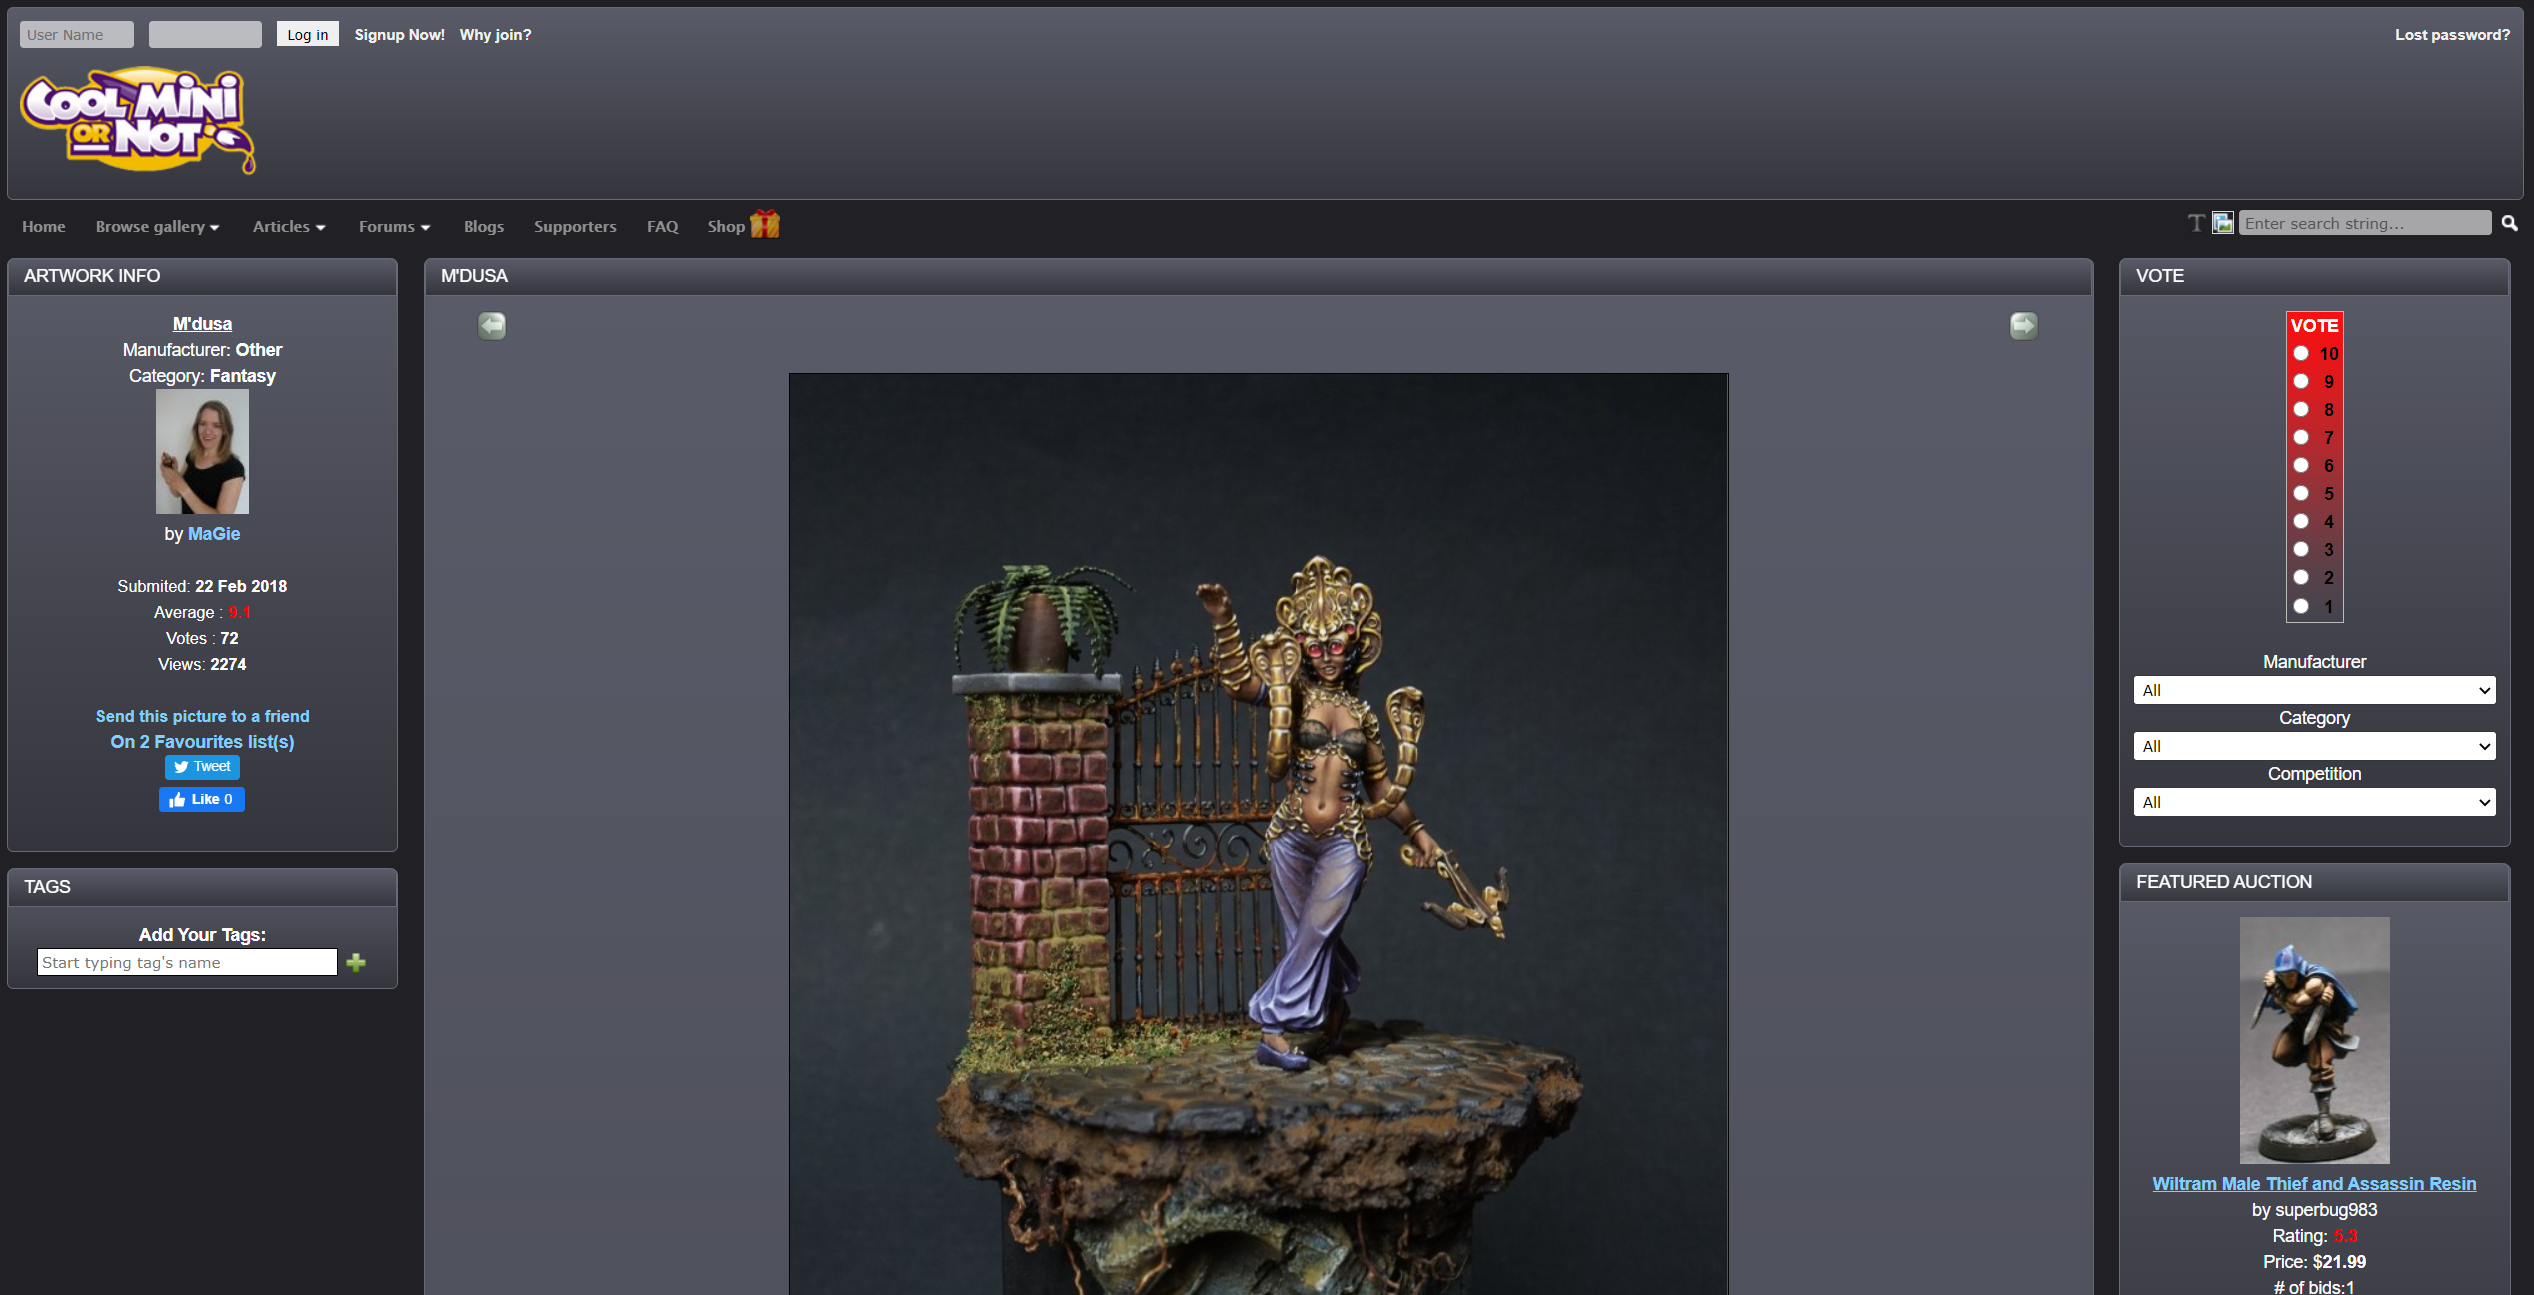
\includegraphics[width=1.0\columnwidth]{pics/page_submission.png}
\caption{Coolmini feltöltés}
\end{figure}

\begin{figure}[H]
\centering
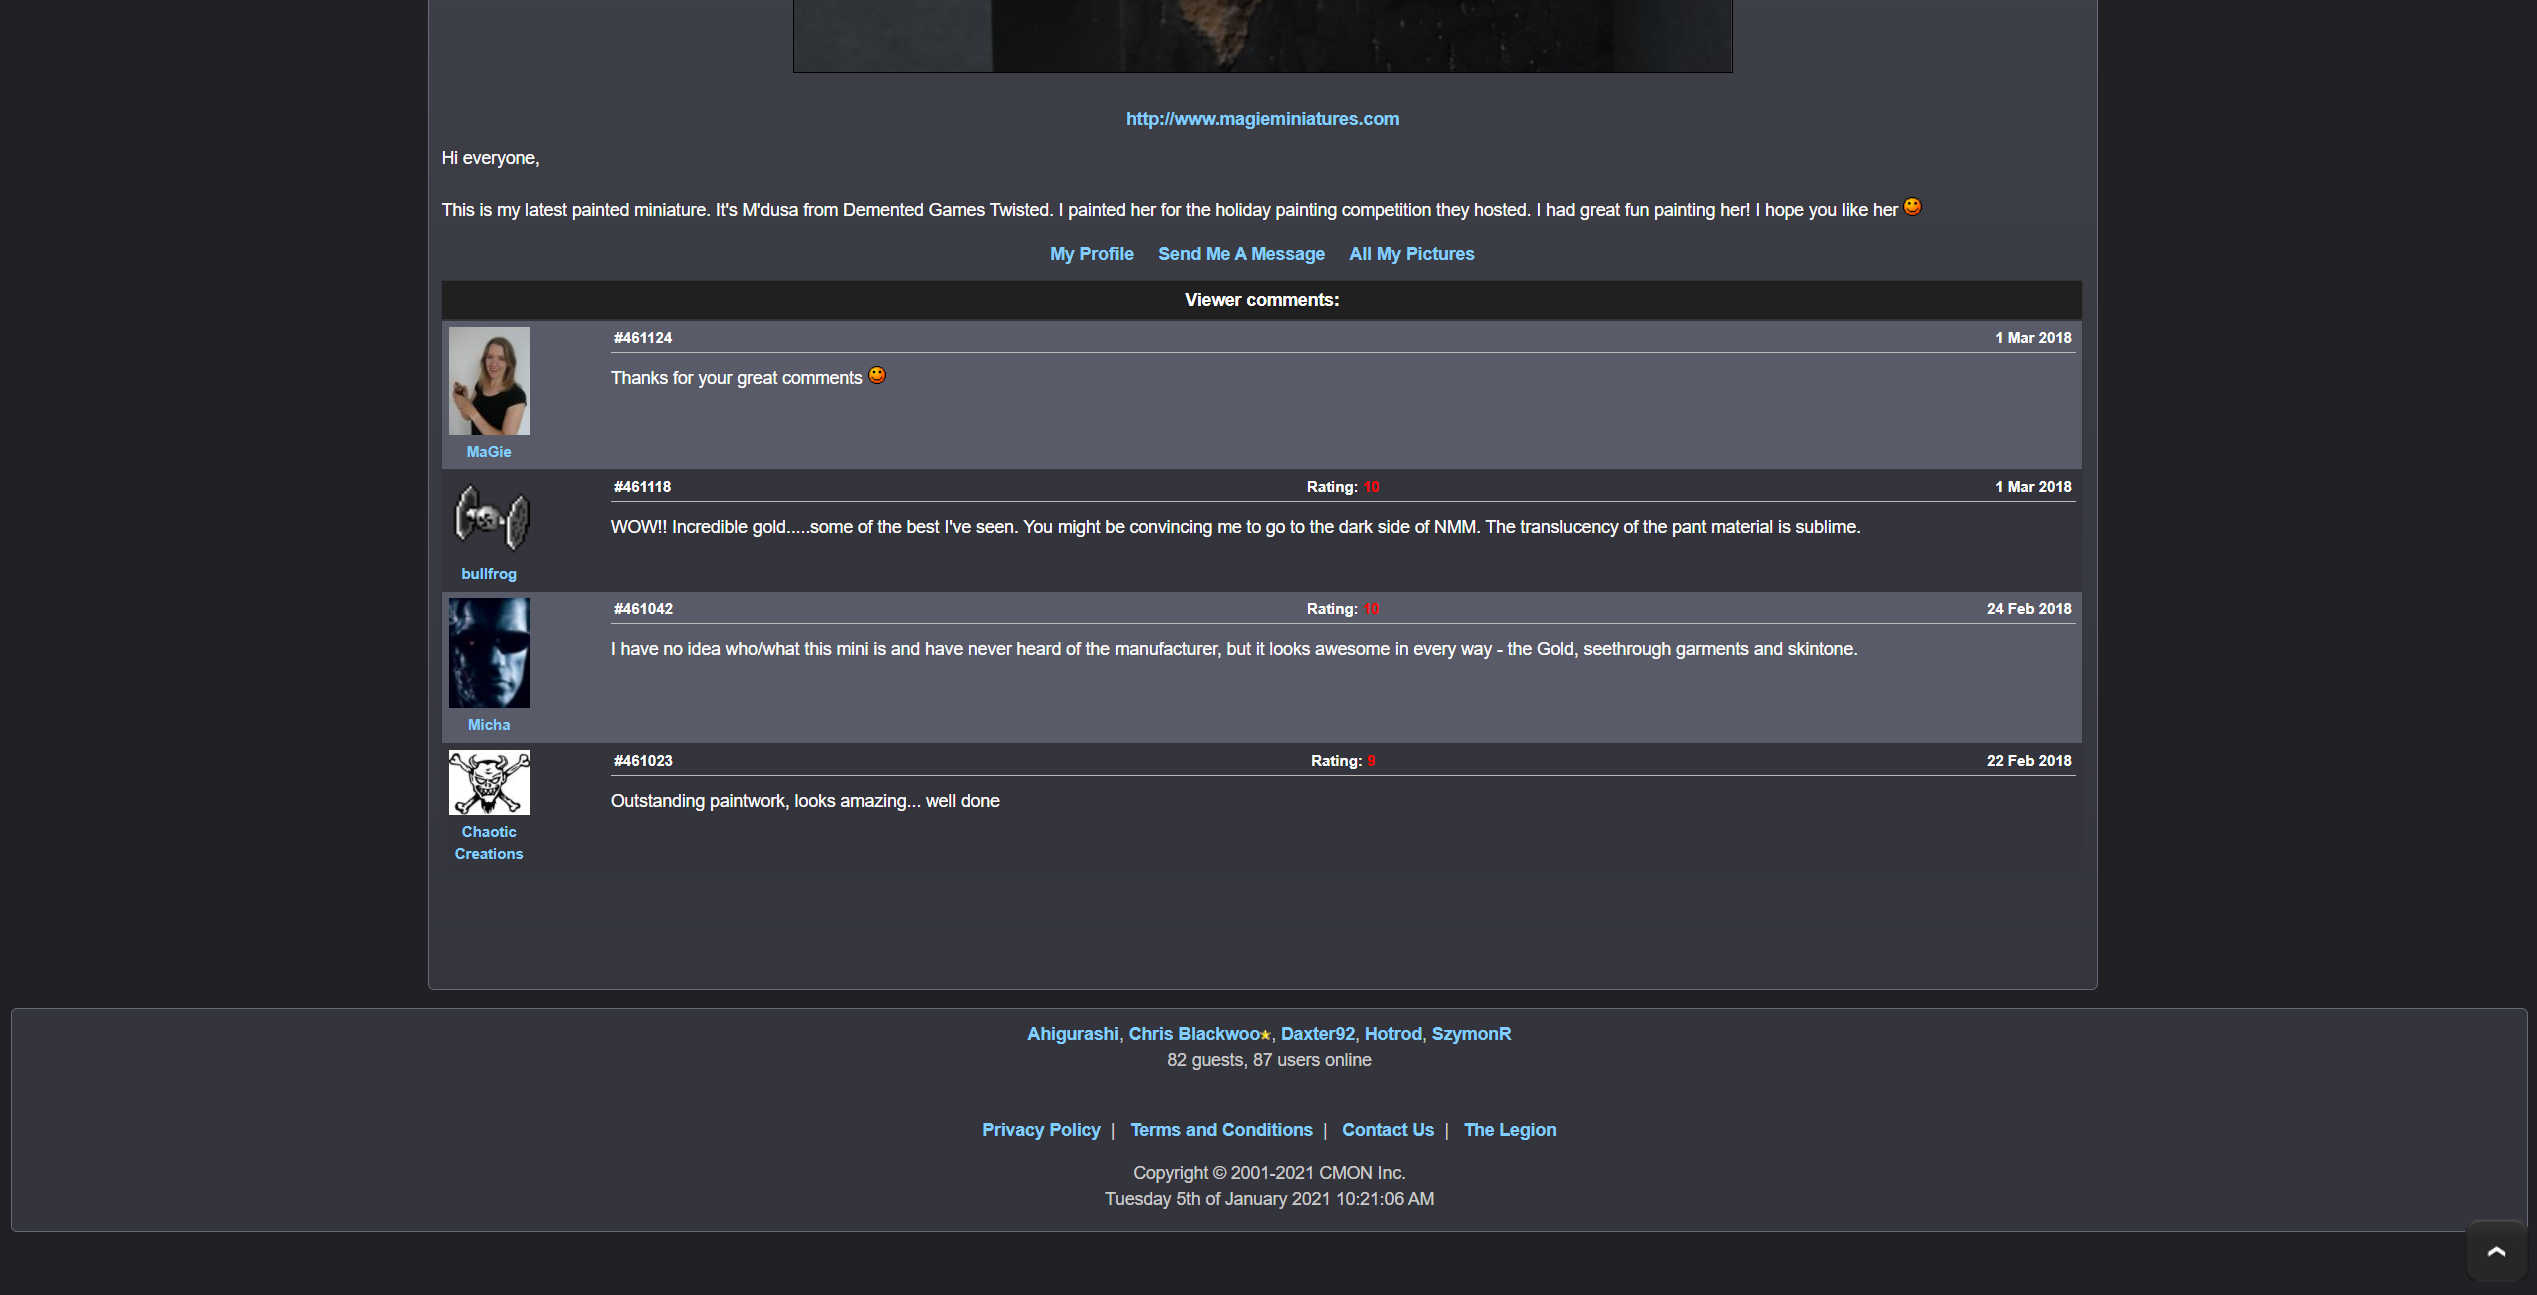
\includegraphics[width=1.0\columnwidth]{pics/page_comments.png}
\caption{Coolmini feltöltés}
\end{figure}

\section{Adathalmaz letöltése}

Az első feladat a weboldal adatainak a kinyerése volt. Ez általában egy nehézkes és körülményes feladat. Nagy
méretű adathalmazról van szó, több 10 GB-nyi adat, melyet napokon keresztül tudunk csak letölteni. Általában a
weboldalak üzemeltetői nem szeretik az ilyen jellegű letöltéseket, ezért előfordulhat, hogy blokkolják az IP
címünket (például DDOS támadásnak hiszik a letöltést).

Szerencsére azonban a weboldal tartalma archiválva lett a Wayback Machine által (\url{https://web.archive.org/web/2020*/coolminiornot.com}), ehhez pedig már létezik letöltő script (\url{https://github.com/hartator/wayback-machine-downloader}).

A letöltő scriptet Raspberry Pi-n keresztül futtattam, mivel összesen 2 héten keresztül tartott a letöltés.

Sajnos problémát jelentett, hogy bizonyos régebbi bejegyzések rossz formátumban töltődtek le az oldalról, ezért egyéb
letöltési lehetőségekkel is próbálkoztam (wget), azonban ezekben az esetekben a felhasználók kommentjeit nem lehetett
letölteni, ezért végül az eredeti adathalmazt használtam fel, a hibás fájlok kiszűrésével.

\section{Transzformáció}

A következő feladat az adatok kinyerése volt a HTML fájlokból. Ehhez az LXML nevű Python modult használtam, melynek segítségével XML fájlokat lehet parsolni. A következő python program segítségével készítettem el az adathalmazt:

\inputminted[linenos, breaklines, fontsize=\footnotesize]{python}{../python/process.py}

\end{document}


